%% LyX 1.6.5 created this file.  For more info, see http://www.lyx.org/.
%% Do not edit unless you really know what you are doing.
\documentclass[english]{article}
\usepackage[T1]{fontenc}
\usepackage[latin9]{inputenc}
\usepackage{float}
\usepackage{amstext}
\usepackage{graphicx}
\usepackage{esint}
\usepackage{babel}

\begin{document}
Diffraction grating is an optical component with a periodic structure.
This component is of interest because any light beam that strike it,
is defleted into discrete angles that depends on the light wavelength.
If the light is composed of light of different wavelengths. A diffraction
grating would send each component to a different direction. Allowing
us to estimate the amount of light of each wavelength. This effect
resambles a Fourier analysis where the harmonic component of a function
is evaluated. Here we shall show that such resemblance is not fortuitous.
What the limitations of such resemblance are.

\[
F\left(\nu,\tau\right)=\delta t\sum_{n=-\infty}^{\infty}S\left(\tau\right)R\left(t-n\delta t\right)e^{-i2\pi\nu\delta t}\]


\[
F_{\nu}=\int_{-\infty}^{\infty}S\left(t\right)e^{i2\pi t\nu}\]


We can show that a diffraction grating perform such an operation,
in fact, we imply that any filtering device performs this operation.
First we shall observe that the above operation is performed over
a infinite range. Which is not possible practically. We shall then
analyse the case if the integration is done in a time span $T$, this
change however introduces a degree of freedom to what the starting
time of integration, the integral is no more unique. We shall then
index each integral by the integration starting point, leading us
to\[
F_{\nu}\left(t\right)=\int_{-\infty}^{\infty}R\left(t-\tau\right)S\left(\tau\right)e^{i2\pi\tau\nu}d\tau,\]
 where at $R$ is a rectangle pulse function. The $R$ function can
be loosen to any square integrable function.

\[
\]
 \[
E_{out}\left(t\right)=\int_{-\infty}^{\infty}R\left(t-\tau\right)E\left(\tau\right)d\tau\]
 \[
E^{2}\]
 \[
\int_{-\infty}^{\infty}DR\left(t-\tau\right)S\left(\tau\right)d\tau\int_{-\infty}^{\infty}DR\left(\tau'\right)S\left(t-\tau'\right)d\tau'\]
 \[
\left|Out\right|^{2}=\]
 \[
FT\left(Out^{2}\right)=\]
 \[
DR\left(t\right)=\sum\delta\left(t-n\delta t\right)R\]


\[
FT\left(Out\right)=HG\]
 %
\begin{figure}
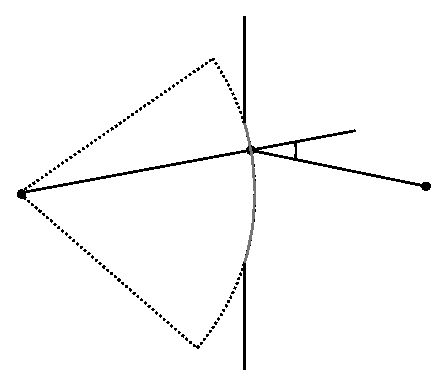
\includegraphics{aperture_diffraction}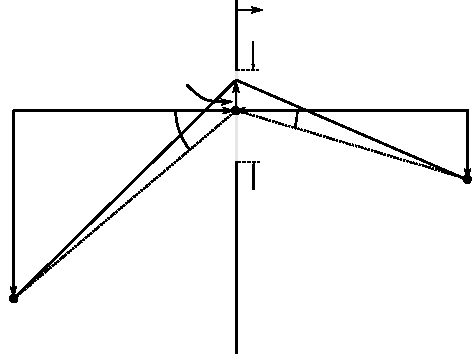
\includegraphics{aperture_coord}\caption{}


\label{fig:aperture}
\end{figure}


To stabilish the terminology we give a brief review of diffraction
theory. Starting with Huygens principle that states that each point
of a wavefront is a new wave source. With such principle in mind.
The problem of the diffraction by a small aperture, depicted at figure
\ref{fig:aperture}, can seen in the following way. If wave are generated
by a point source $P_{0}$ at a point $Q$ the wave field should be\[
E\left(Q\right)=E\left(P_{0}\right)\frac{e^{ikr}}{r},\]
 where $r$ the distance between $P_{0}$ and $Q$, and $k$ is the
wavenumber. The field at a point $P$ due to source at $Q$ is then\[
E\left(P\right)=E\left(P_{0}\right)\frac{e^{ikr}}{r}\frac{e^{iks}}{s}K\left(\chi\right),\]
 where $K\left(\chi\right)$ an inclination factor which describes
the variation with direction of the amplitude of the secondary waves,
$\chi$ been the angle between the primary wavefront normal and the
direction of $QP$. The at $P$ due to all wave sources at surface
$S$ will then be\begin{equation}
E\left(P\right)=E\left(P_{0}\right)\int_{S}\frac{e^{ikr}}{r}\frac{e^{iks}}{s}K\left(\chi\right)dS.\label{eq:huygens formula}\end{equation}


The Huygens principle was then put on a sounder mathematical basis
by Kirchhoff\foot{Section 8.3 Born and Wolf}. Using Green's theorem
on the time-independent wave equation\[
\left(\nabla^{2}+k^{2}\right)E=0,\]
 one can derive that\[
E\left(P\right)=\frac{1}{4\pi}\int_{S}\left[E\left(Q\right)\frac{\partial}{\partial n}\left(\frac{e^{iks}}{s}\right)-\frac{e^{iks}}{s}\frac{\partial E}{\partial n}\left(Q\right)\right]dS,\]
 where $\partial/\partial n$ is the differentiation along the normal
to $S$. This one form of the integral theorem of Helmoktz and Kirchhoff.
Since $\frac{\partial}{\partial n}\left(\frac{e^{iks}}{s}\right)=\frac{e^{iks}ik}{s}\left[1-\frac{1}{iks}\right]\cos\left(n,s\right)$,
considering that $ks\gg1$\[
E\left(P\right)=\frac{1}{4\pi}\int_{S}\frac{e^{iks}}{s}\left[ikE\left(Q\right)\cos\left(n,s\right)-\frac{\partial E}{\partial n}\left(Q\right)\right]dS,\]


For a point source at $P_{0}$ the field at $Q$ is $E\left(Q\right)=E\left(P_{0}\right)\frac{e^{iks}}{s}$.
The Fresnel-Kirchoff formula will be\[
E\left(P\right)=\int_{S}E\left(P_{0}\right)\frac{-ik}{4\pi}\frac{e^{ikr}}{r}\frac{e^{iks}}{s}\left[\cos\left(n,r\right)-\cos\left(n,s\right)\right]dS,\]
 Which is known as the Fresnel-Kirchhoff diffraction formula. since
$\cos\left(n,r\right)=1$ and $\left(n,s\right)=\pi-\chi$ the above
integral is\[
E\left(P\right)=E\left(P_{0}\right)\int_{S}\frac{e^{ikr}}{r}\frac{e^{iks}}{s}\frac{-ik}{4\pi}\left(1+\cos\chi\right)dS.\]
 Which validates the Huygens principle. Comparing with \ref{eq:huygens formula}
we note that\[
K\left(\chi\right)=\frac{-ik}{4\pi}\left(1+\cos\chi\right).\]


A special case of the Fresnell-Kirchhoff diffraction formula is the
Fraunhofer diffraction, in this case, the diffracting element is much
smaller than the distances where the field is being evaluated. Figure
X, depict such case. Where the assumption is that $\frac{W}{r}$ and
$\frac{W}{s}\ll1$. In such case we have that\[
s'\approx s+\xi\sin\theta\]
 \[
r'\approx r+\xi\sin\theta_{0}\]


Which will cause the Fresnel-Kirchhoff formula to be approximated
to\[
E\left(P\right)=C\int_{-W/2}^{W/2}e^{ik\xi\left(\sin\theta_{0}+\sin\theta\right)}d\xi,\]
 where $C=E\left(P_{0}\right)\frac{-ik}{4\pi}\frac{e^{ikr}}{r}\frac{e^{iks}}{s}\left(\cos\theta-\cos\theta_{0}\right)$\[
E_{\text{aperture}}=CW\text{sinc}\left[\left(\sin\theta_{0}+\sin\theta\right)\frac{Wk}{2\pi}\right].\]


For a grating with period $d$ and aperture $w$ the integral will
be\[
\sum_{n}\int_{nd-W/2}^{nd+W/2}e^{ik\xi\left(\sin\theta_{0}+\sin\theta\right)}d\xi,\]
 with transformation of variable $\xi=\xi'-nd$\[
\sum_{n}\int_{-W/2}^{W/2}e^{ik\left(\xi'-nd\right)\left(\sin\theta_{0}+\sin\theta\right)}d\xi'\]
 \[
\int_{-W/2}^{W/2}e^{ik\xi'\left(\sin\theta_{0}+\sin\theta\right)}d\xi'\sum_{n}e^{-iknd\left(\sin\theta_{0}+\sin\theta\right)}\]
 \[
E_{\text{grating}}=E_{\text{aperture}}\sum_{n}e^{-iknd\left(\sin\theta_{0}+\sin\theta\right)},\]
 Hence \[
I=\left|E\right|^{2}=I_{\text{aperture}}\left\{ \frac{\sin\left[N\frac{kd}{2}\left(\sin\theta_{0}+\sin\theta\right)\right]}{\sin\left[\frac{kd}{2}\left(\sin\theta_{0}+\sin\theta\right)\right]}\right\} ^{2}\]
 \[
\frac{d}{\lambda}\left(\sin\theta_{0}+\sin\theta\right)=m\]


%
\begin{figure}[h]
\caption{Diffraction grating cross section.}

\end{figure}


A diffraction grating may be defined as any arrangement which imposes
on an incident wave a periodic variation of amplitude of phase, or
both. We may characterize any particular grating by its \emph{transmission
function}\footcite{Born:2000p1607}, defined as follows:

The ratio $\left|V/V_{0}\right|$ is practically unity for points
outside the geometrical shadow (whose boundary is represented by points
A and B in Figure) cast by the object. If the portion outside the
shadow region is covered by an opaque screen, the arrangements act
as a diffracting aperture A with a nonuniform pupil function. 

%
\begin{figure}[H]
 \center{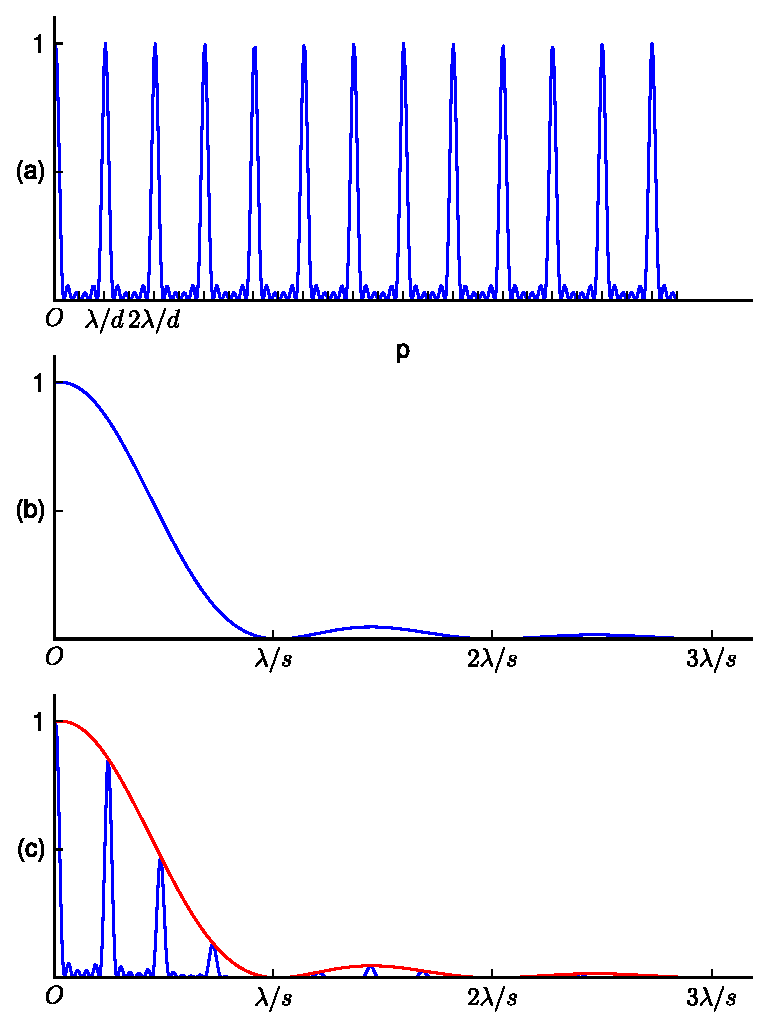
\includegraphics[scale=0.9]{diffraction-grating-basic}}\caption{}

\end{figure}


%(a) The normalized interference function\begin{equation}
%\frac{1}{N^{2}}H\left(N,kdp/2\right)=\left[\frac{\sin\left(Nkdp/2\right)}{N\sin\left(kdp/2\right)}\right]^{2}.\end{equation}
%(b) The normalized intensity function of a slit\begin{equation}
%I^{\left(0\right)}\left(p\right)=\left[\frac{\sin ksp/2}{ksp/2}\right]^{2}.\end{equation}
%(c) The normalized intensity function of a grating consisting of $N$
%similar equidistant parallel slits\begin{equation}
%\frac{1}{N^{2}}I\left(p\right)=\left[\frac{\sin\left(Nkdp/2\right)}{N\sin\left(kdp/2\right)}\right]^{2}\left[\frac{\sin ksp/2}{ksp/2}\right]^{2}.\end{equation}
%Only the range $p\ge0$ is shown, all the curves being symmetrical
%about the vertical axis $p=0$.


Let us now consider a one-dimensional grating consisting of $n$ parallel
grooves of arbitrary profile, ruled on one surface of a plan-parallel
glass plate. Let the $\xi,\eta$-plane coincide with the plane face
of the plate, $\eta$ being the direction of the grooves and let $d$
be the period in the $\xi$ direction.

Assume that the direction of propagation of the wave incident upon
the grating is in the plane of the figure, making an angle $\theta_{0}$
with $O\zeta$, and let $\theta$ denote the angle which $O\zeta$
makes with the line joining a very distant point of observation P
with the grating.

As before we set $l_{o}=\sin\theta_{0}$, $l=\sin\theta$, $p=l-l_{0}=\sin\theta-\sin\theta_{0}$.
The complex amplitude at $P$ is then immediately obtained from, where
the integrand must be multiplied by the transmission function $F$
of one periodic element. We may set $q=0$ and\begin{equation}
\begin{array}{ccc}
\xi_{n}=nd, & \eta_{n}=0 & \left(n=0,1,\ldots,N-1\right)\end{array}.\end{equation}
 We the obtain\begin{equation}
U\left(p\right)=U^{\left(0\right)}\left(p\right)\sum_{n=0}^{N-1}e^{-ikndp}=U^{\left(0\right)}\left(p\right)\frac{1-e^{-iNkdp}}{1-e^{-kdp}},\label{eq: Up}\end{equation}
 where\begin{equation}
U^{\left(0\right)}\left(p\right)=C\int_{A}\! F\left(\xi\right)e^{-ikp\xi}\, d\xi.\label{eq: diffraction envelope}\end{equation}
 Hence\begin{equation}
I\left(p\right)=\left|U\left(p\right)\right|^{2}=\frac{\left(1-e^{-Nkdp}\right)}{\left(1-e^{-kdp}\right)}\cdot\frac{\left(1-e^{Nkdp}\right)}{\left(1-e^{kdp}\right)}\left|U^{\left(0\right)}\left(p\right)\right|^{2}=\frac{1-\cos Nkdp}{1-\cos kdp}I^{\left(0\right)}\left(p\right),\end{equation}
 where $I^{\left(0\right)}\left(p\right)=\left|U^{\left(0\right)}\left(p\right)\right|^{2}$.
If we introduce the function\begin{equation}
H\left(N,x\right)=\left(\frac{\sin Nx}{\sin x}\right)^{2},\end{equation}
 the formula 5 for the intensity may be written as\begin{equation}
I\left(p\right)=H\left(N,\frac{kdp}{2}\right)I^{\left(0\right)}\left(p\right).\end{equation}
 Before discussing the implications of this basic formula we note
that according to \ref{eq: Up}. The light distribution is the same
as that due to a set of coherent secondary sources each characterized
by the same amplitude function $\left|U^{\left(0\right)}\left(p\right)\right|$
and with phases that differ form each other by integral multiples
of $kdp$. To see the significance of this phase difference consider
two corresponding points $A$ and $B$ in the neighboring grooves
of the grating. Since the effect of the grating is to impress a periodic
variation onto the incident wave, it follows that the path difference
between the light arriving a $A$ and at $B$ is the same as in the
absence of the grating, i.e. it is equal to $AK=d\sin\theta_{0}$,
$K$ denoting the foot of the perpendicular from $B$ on to the ray
incident at $A$. Further, the light path from $B$ in the direction
$\theta$ exceeds the light path from $A$ by $BL=d\sin\theta$, $L$
being the foot of the perpendicular from $A$ on to the ray diffracted
at $B$ in the direction $\theta.$ Hence the total path difference
between light arriving at the distant point of observation form corresponding
points in two neighboring grooves is\begin{equation}
BL-AK=d\left(\sin\theta-\sin\theta_{0}\right)=dp,\label{eq: path difference}\end{equation}
 and the corresponding phase difference is $2\pi dp/\lambda=kdp$.

Formula expresses $I\left(p\right)$ as the product of two functions:
one of them, $I^{\left(0\right)}$, represents the effect of a single
period of the grating; the other, $H\left(N,x\right)$ has maxima,
each of height $N^{2}$ when\begin{equation}
p\equiv\sin\theta-\sin\theta_{0}=\frac{m\lambda}{Nd}\left(m=0,\pm1,\pm2,\ldots\right),\label{eq:grating equation}\end{equation}
 The integer $m$ represents, according to 7, the path difference
in wavelengths between light diffracted in the direction of the maximum,
from corresponding points in two neighboring grooves. In agreement
with our earlier definition,7.3.1, we call $m$ the \emph{order of
interference}. Between theses principal maxima there are weak secondary
maxima (see fig 8.19a), the first secondary maximum being only a few
percent of the principal maximum when $N$ is large. The maxima are
separated by points of zero intensity at $x=kdp/2=\pm n\pi/N$, i.e.
in directions given by\begin{equation}
p\equiv\sin\theta-\sin\theta_{0}=\frac{n\lambda}{Nd}\left(n=0,\pm1,\pm2,\ldots\right)\label{eq: grating secondary maxima}\end{equation}
 the case where $n/N$ is an integer being excluded.

The function $I^{\left(0\right)}\left(p\right)$ depends on the form
of the grooves. Suppose that it has principal maximum for some direction
$p=p'$ and that on both sides of the maximum if falls off slowly
in comparison with $H$. Then $I\left(p\right)$ will have the general
form o the sharp maxima near the directions $p=m\lambda/d$. Since
these directions (except for $m=0$) depend on the wavelength, we
see that the grating will decompose a beam of non-monochromatic light
into \emph{spectral orders}.

To illustrate these remarks let us consider a grating consisting of
a succession of long equidistant slits, each of width $s$ and length
$L$, in an opaque screen. If the grating is illuminated from a very
distant line source parallel to the slits, the intensity $I^{\left(0\right)}$
is given by the expression \ref{eq: diffraction envelope} (with $2a=s$,
$2b=L$) and we obtain\begin{equation}
I\left(p\right)=\frac{sE}{\lambda R^{2}}\left(\frac{\sin\frac{Nkdp}{2}}{\sin\frac{kdp}{2}}\right)^{2}\left(\frac{\sin\frac{kdp}{2}}{\frac{kdp}{2}}\right)^{2}.\label{eq: diffraction intensity}\end{equation}
 Curves representing the two factors in \ref{eq: diffraction intensity}
and their product are shown in fig X. The last factor in \ref{eq: diffraction intensity},
which represents the effect of a single slit, has a principal maximum
at $p=0$ and minima given by $ksp/2=n\pi$, i.e. at\begin{equation}
p=\frac{n\lambda}{s},\left(n=0,\pm1,\pm2,\ldots\right)\end{equation}
 separated by weak secondary maxima. We see that if $\lambda/s\gg\lambda/d$,
i.e. if the width of each slit is small compared to $d$, the intensity
$I\left(p\right)$ has in addition to a principal maximum at $p=0$
a series of sharp, but progressively decreasing, maxima on either
side of it, near direction given by \ref{eq:grating equation}.

Returning to the general case, it is evident that if the width of
each groove is very small, of the order of a wavelength (as is often
the case in practice) the formula derived on the basis of Kirchhoff's
approximation, can evidently no longer be expected to hold. In such
cases more refined considerations must be make to determine the detailed
distribution of the intensity. We may, however, expect that the main
qualitative features indicated by our elementary theory, namely the
existence of sharp maxima whose positions are substantially determined
by the interference function $H$, remain even when the grooves are
very narrow, provided, that the intensity function of a single period
varies slowly in an interval of the order $\Delta p=\lambda/d$. Let
us now consider the resolution that may be attained with a grating.
The separation between a primary maximum of order $m$ and a neighboring
minimum is, according to \ref{eq: grating secondary maxima}, given
by\begin{equation}
\Delta p=\frac{\lambda}{Nd}.\end{equation}
 If the wavelength is changed by an amount $\Delta\lambda$, the $m$th-order
maximum is according to \ref{eq:grating equation}, displaced by an
amount\begin{equation}
\Delta'p=\frac{\left|m\right|}{d}\Delta\lambda.\end{equation}
 Assuming that the lines of wavelength $\lambda\pm\frac{1}{2}\Delta\lambda$
will just be resolved when the maximum of the one wavelength coincides
with the first minimum of the other we have on he limit of resolution
in the $m$th order, $\Delta p=\Delta'p$, i.e.\begin{equation}
\frac{\lambda}{\Delta\lambda}=\left|m\right|N.\label{eq: resolving power}\end{equation}
 Thus, \emph{the resolving power is equal to the product of the order
number m and the number N of the grooves}. For the $m$th order we
have, according to, that $d\left(\sin\theta-\sin\theta_{0}\right)=m\lambda$,
so that we may also express the resolving power in the form\begin{equation}
\frac{\lambda}{\Delta\lambda}=\frac{Nd\left|\sin\theta-\sin\theta_{0}\right|}{\lambda}.\end{equation}
 Because of \ref{eq: path difference} this implies that \emph{the
resolving power is equal to the number of wavelengths in the path
difference between rays that are diffracted in the direction $\theta$
from the two extreme ends (separated by distance Nd) of the grating}.
It is to be noted that since $\left|\sin\theta-\sin\theta_{0}\right|$
cannot exceed 2, the resolving power that can be attained with a grating
of overall with $w$ can never exceed the value $2w/\lambda$.
\end{document}
